\section{Selected} \label{sec:Selected}

This utility creates a new coordinate file. By default, the utility saves all
bead and molecules types (basically transforming one coordinate file format into
another), but there are options to fine-tune what is excluded or kept (\tt{-bt},
\tt{-mt}, \tt{--keep}, \tt{-cx/y/z}). There are also some basic manipulations
for the coordinates from connecting molecules split via periodic boundary
conditions or wrapping beads back into the box (\tt{--join}, \tt{--keep}) to
scaling coordinates or moving particles (\tt{-sc}, \tt{-m}).

\subsubsection*{Selecting bead and/or molecule types to exclude or keep}

The \tt{-bt} and \tt{-mt} options select bead and molecule types, respectively.
By default, the selected types are excluded (i.e., all other types are saved
into the output file); the \tt{--keep} option reverses the behaviour (i.e., only
the selected types are saved).

\begin{table}[h]
  \caption{
    Interactions of \tt{-bt}, \tt{-mt}, and \tt{--keep} options when used on a
    system containing bead types that are both unbonded and in molecules. For
    molecule types, the name represents initial composition (e.g., \tt{ABC}
    comprises 1 bead of each of \tt{A}, \tt{B}, and \tt{C} bead types), and the
    brackets show the final composition of the molecule (e.g., 1~(no \tt{B}) for
    \tt{ABC} molecule means only \tt{A} and \tt{C} beads remain in the
    molecule). For bead types, $a+b$ indicates unbonded beads ($a$) and beads in
    molecules ($b$).
  }\label{tab:Selected-btmtkeep}
  \centering
  \begin{tabular}{lcccccc}
    \toprule
    \multirow{2}{*}{Options used on \enquote{full}}
    & \multicolumn{3}{c}{Molecule types} & \multicolumn{3}{c}{Bead types} \\
    \cmidrule(lr){2-4} \cmidrule(lr){5-7}
                             & ABC        & AB       & AC & A    & B    & C\\
    \midrule
    full                     & 1          & 1        & 1 & 10+3 & 10+2 & 10+2\\
    \cmidrule(lr){1-7}
    \tt{-bt B}               & 1 (no B)   & 1 (no B) & 1 & 10+3 & 0    & 10+2\\
    \tt{-bt B -mt AB}        & 1 (no B)   & 0        & 1 & 10+2 & 0    & 10+2\\
    \tt{-bt B -mt AB --keep} & 1 (only B) & 1        & 0 & 0+2  & 10+2 & 0\\
    \bottomrule
  \end{tabular}
\end{table}

\Cref{tab:Selected-btmtkeep} shows possible interactions between the three
options when some beads are unbonded and other beads of the same type are in a
bond. The \enquote{full} system is in the \tt{Examples/Selected} directory as
the \tt{full.vtf} file.

\subsubsection{Constraining and manipulating coordinates}

The \tt{-cx}, \tt{-cy}, and \tt{-cz} options constrain beads to be saved to
specified coordinate ranges (by default, the range is in fractions of the
simulation box). The options accept multiples of number pairs for each axis; a
bead coordinate must fall within at least one of the ranges, e.g., using \tt{-cx
0 0.1 0.9 1} would save beads whose $x$ coordinates are within 0 to 10\% or
90\% to 100\% of the box size in the x-direction. Adding, e.g., \tt{-cy 0.4
0.6} would save only the beads that fulfil the \tt{-cx} option as well as this
one, i.e., that $y$ coordinate is between 40\% and 60\% of the simulation box.

The \tt{-sc <float>} option scales all coordinates by dividing them via the
specified number.

The \tt{-m <x> <y> <z>} option moves all coordinates by the specified vector (by
default, the vector is in fractions of simulation box).

If multiple options are used, they manipulate the coordinates in the order
\tt{-cx/y/z}, \tt{-sc}, \tt{-m}, i.e. first, coordinates are constrained, then
scaled, and lastly moved. See \cref{fig:Selected} for an example: if all three
options are specified in one command, it transforms the \enquote{original}
system in the direction of \enquote{all options at once} with the beads ending
up outside the box. This is equivalent to running three consecutive commands,
first only with \tt{-cx/y/z} (from \enquote{original} system to the right), then
with \tt{-sc} (down), and lastly with \tt{-m} (left). \Cref{fig:Selected} shows
what happens when the \tt{Selected} commands are run in different order. These
examples are also in the \tt{Examples/Selected} directory.

As mentioned above, both \tt{-cx/y/z} and \tt{-m} options accept fractions of
box size (i.e., numbers between 0 and 1) by default. To specify \enquote{real}
coordinates instead, use the \tt{--real} option.

Note that neither of these options changes the size of the simulation box.

\begin{figure}[t]
  \centering
  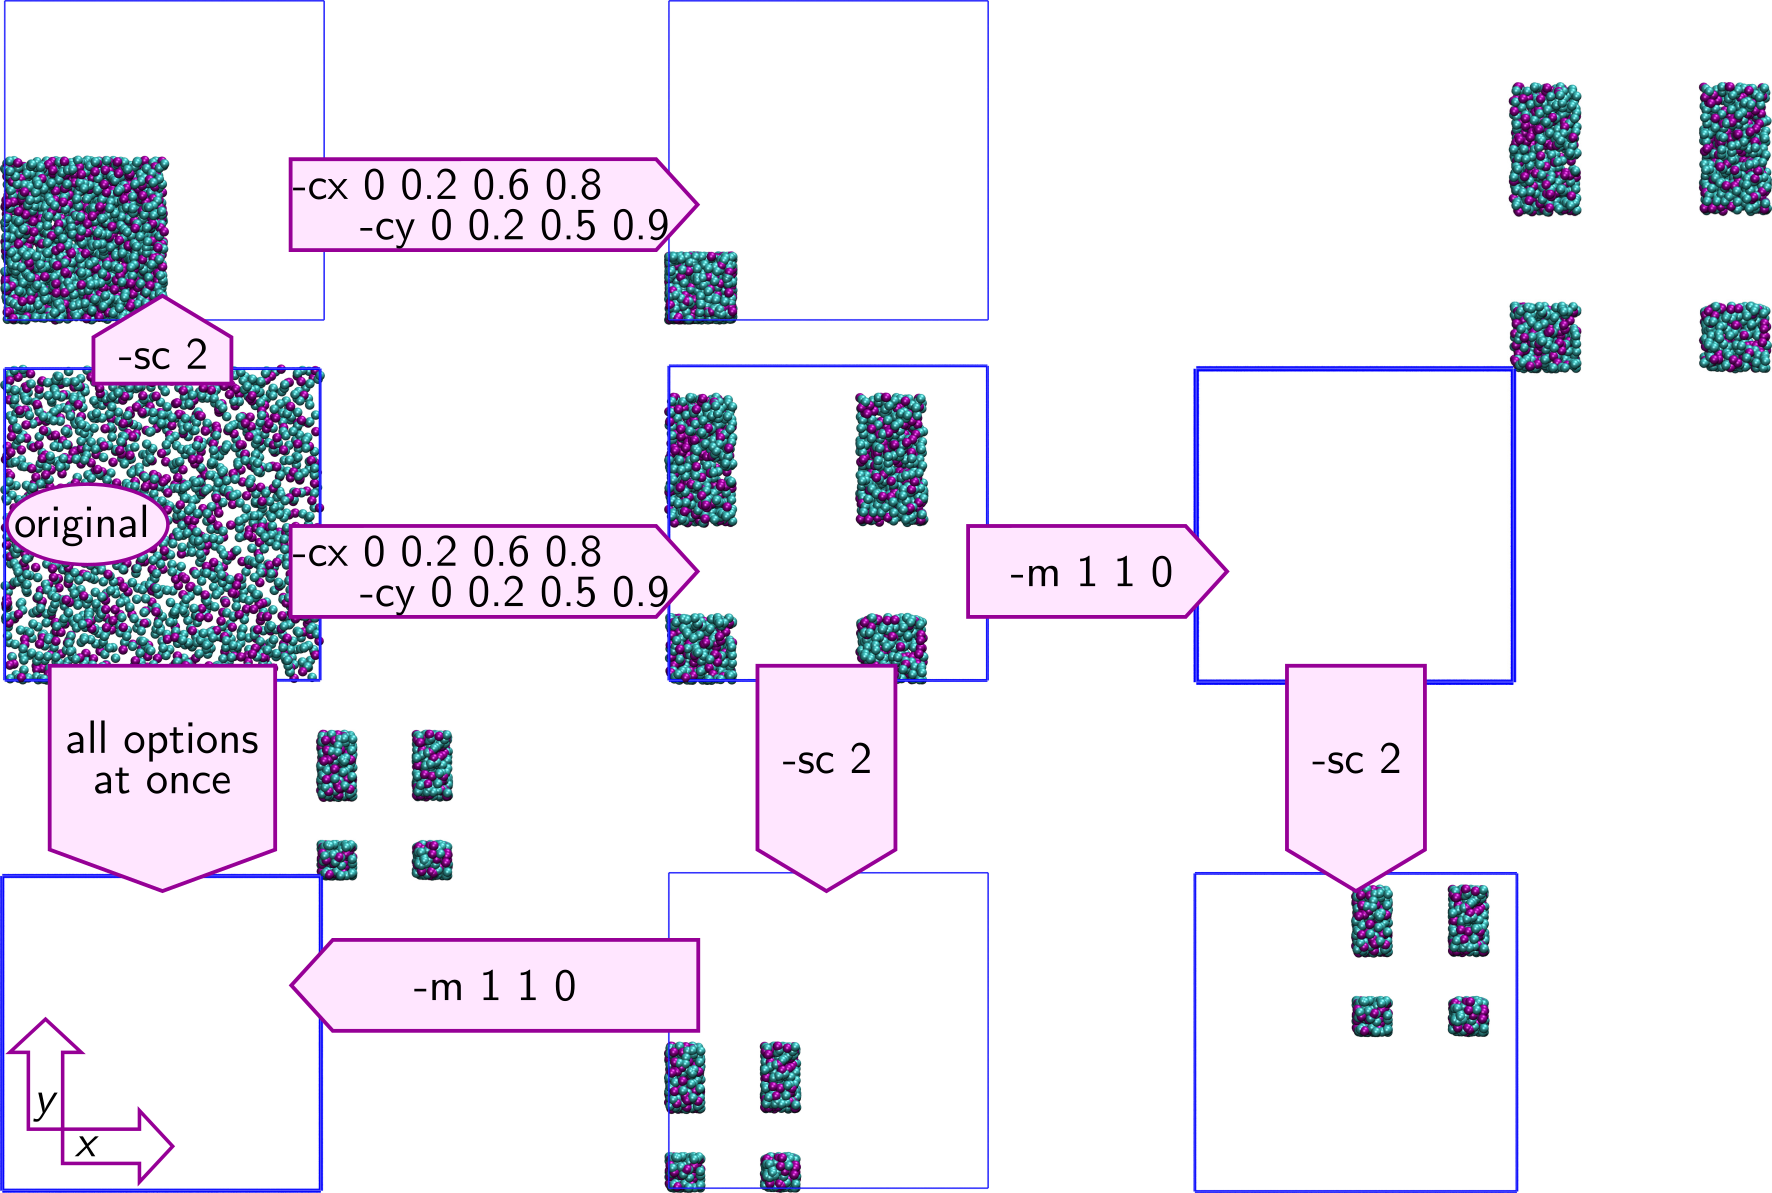
\includegraphics{Selected.png}
  \caption{
    Some of the possible results when combining sequential runs of the
    \tt{Selected} utility, namely (1) constraining $x$ and $y$ coordinates via
    \tt{-cx 0 0.2 0.6 0.8 -cy 0 0.2 0.5 0.9}, (2) scaling (dividing) coordinates
    via \tt{-sc 2}, and (3) moving coordinates via \tt{-m 1 1 0}. The blue lines
    represent the simulation box (the varying line thickness is just an
    artefact of how the snapshots were created in \tt{vmd}).
  }
  \label{fig:Selected}
\end{figure}

\subsubsection{Dealing with periodic boundary conditions}

The input system may contain beads that are outside the simulation box. The
\tt{--wrap} option returns all beads into the simulation box\dots

Conversely, molecules can be disconnected due to the periodic boundary
conditions with one part of the molecule on one side of the box and another part
on the opposite side. The \tt{--join} removes the periodic boundary conditions,
making the molecule whole as well as stick out of the simulation box. The centre
of mass of every \enquote{joined} molecule is inside the simulation box.

If both options are specified, the coordinates are first wrapped via \tt{--wrap}
and then the molecules are \enquote{joined} via \tt{--join}.

\vspace{1em}
\noindent
Usage: \tt{Selected <input> <output> <bead type(s)> [options]}
\noindent
\begin{longtable}{p{0.22\textwidth}p{0.724\textwidth}}
  \toprule
  \multicolumn{2}{l}{Mandatory arguments}\\
  \midrule
  \tt{<input>}        & input coordinate file\\
  \tt{<output>}       & output coordinate file\\
  \midrule
  \multicolumn{2}{l}{Options}\\
  \midrule
  \tt{-bt <bead type>} & bead types to exclude\\
  \tt{-mt <mol type>}  & molecule types to exclude\\
  \tt{--keep}          & save only specified types instead of excluding them\\
  \tt{--join}          & join molecules by removing periodic boundary
                         conditions\\
  \tt{--wrap}          & wrap simulation box (i.e., apply periodic boundary
                         conditions)\\
  \tt{-n <int(s)>}     & save only specified timesteps\\
  \tt{--last}          & save only the last step\\
  \tt{-sc <float>}     & divide all coordinates by given value\\
  \tt{-m <x> <y> <z>}  & add specified vector to all coordinates (\tt{-sc} is
                         applied first)\\
  \tt{-cx n×2×<float>} & constrain x-coordinates to specified dimension;
                         multiple pairs possible\\
  \tt{-cy n×2×<float>} & same as \tt{-cx} but with y-coordinates\\
  \tt{-cz n×2×<float>} & same as \tt{-cx} but with z-coordinates\\
  \tt{--real}          & use real coordinates instead of fractions of box size
                         (for \tt{-cx/y/z} and \tt{-m} options)\\
  \midrule
  \multicolumn{2}{l}{Other options (see the beginning of
                     Chapter~\ref{chap:Utils})}\\
  \midrule
  \multicolumn{2}{p{0.948\textwidth}}{\tt{-st},
                                      \tt{-e},
                                      \tt{-sk},
                                      \tt{-i},
                                      \tt{--verbose},
                                      \tt{--silent},
                                      \tt{--help},
                                      \tt{--version}}\\
  \bottomrule
\end{longtable}
